\documentclass[12pt]{article}

%% preambleb
\usepackage{amsmath}
\usepackage[margin = 1in]{geometry}
\usepackage{graphicx}
\usepackage{lipsum}
\usepackage{natbib}

%% meta data

\title{Stats Paper}
\author{Kaitlyn Shevlin\\
  Department of Statistics\\
  University of Connecticut
}

\begin{document}
\maketitle

\begin{abstract}
Here is the abstract.  
\end{abstract}


\section{Introduction}
\label{sec:intro}

Use this section to answer three questions:
Why is the topic important/interesting?
What has been done on this topic in the literature?
What is your contribution?

\lipsum[1-3]

To cite a reference, here are examples.
\citet{xie2015dynamic} did something... \lipsum[1]

A lot of work has been done \citep[e.g.,][]{xie2015dynamic}.
\lipsum[2]
Some parametric bootstrap sample size approach was proposed by
\citet{dwivedi2017analysis}. 


% roadmap
The rest of the paper is organized as follows.
The data will be presented in Section~\ref{sec:data}.
The methods are described in Section~\ref{sec:meth}.
The results are reported in Section~\ref{sec:resu}.
A discussion concludes in Section~\ref{sec:disc}.


\section{Data}
\label{sec:data}

Use this section to describe the data that helps to answer your research questions.
\lipsum{1}

\section{Methods}
\label{sec:meth}

Use this section to present the methodologies that will generate results by
analyzing the data.
\begin{equation}
  \label{eq:line}
  y = 2x + 4 
\end{equation}

Another equation.
\begin{equation}
  \label{eq:line}
y = {1\over\displaystyle x}
\end{equation}


\section{Results}
\label{sec:results}

\begin{table}[ht]
  \caption{This is my first table.}
  \label{tab:rv}
\centering
\begin{tabular}{rrr}
  \hline
Col1 & Col2 & Col3 \\ 
  \hline
1 & 2 & 3 \\ 
4 & 5 & 8\\ 
7 & 8 & 9\\ 
   \hline
\end{tabular}
\end{table}



\begin{figure}
  \centering
  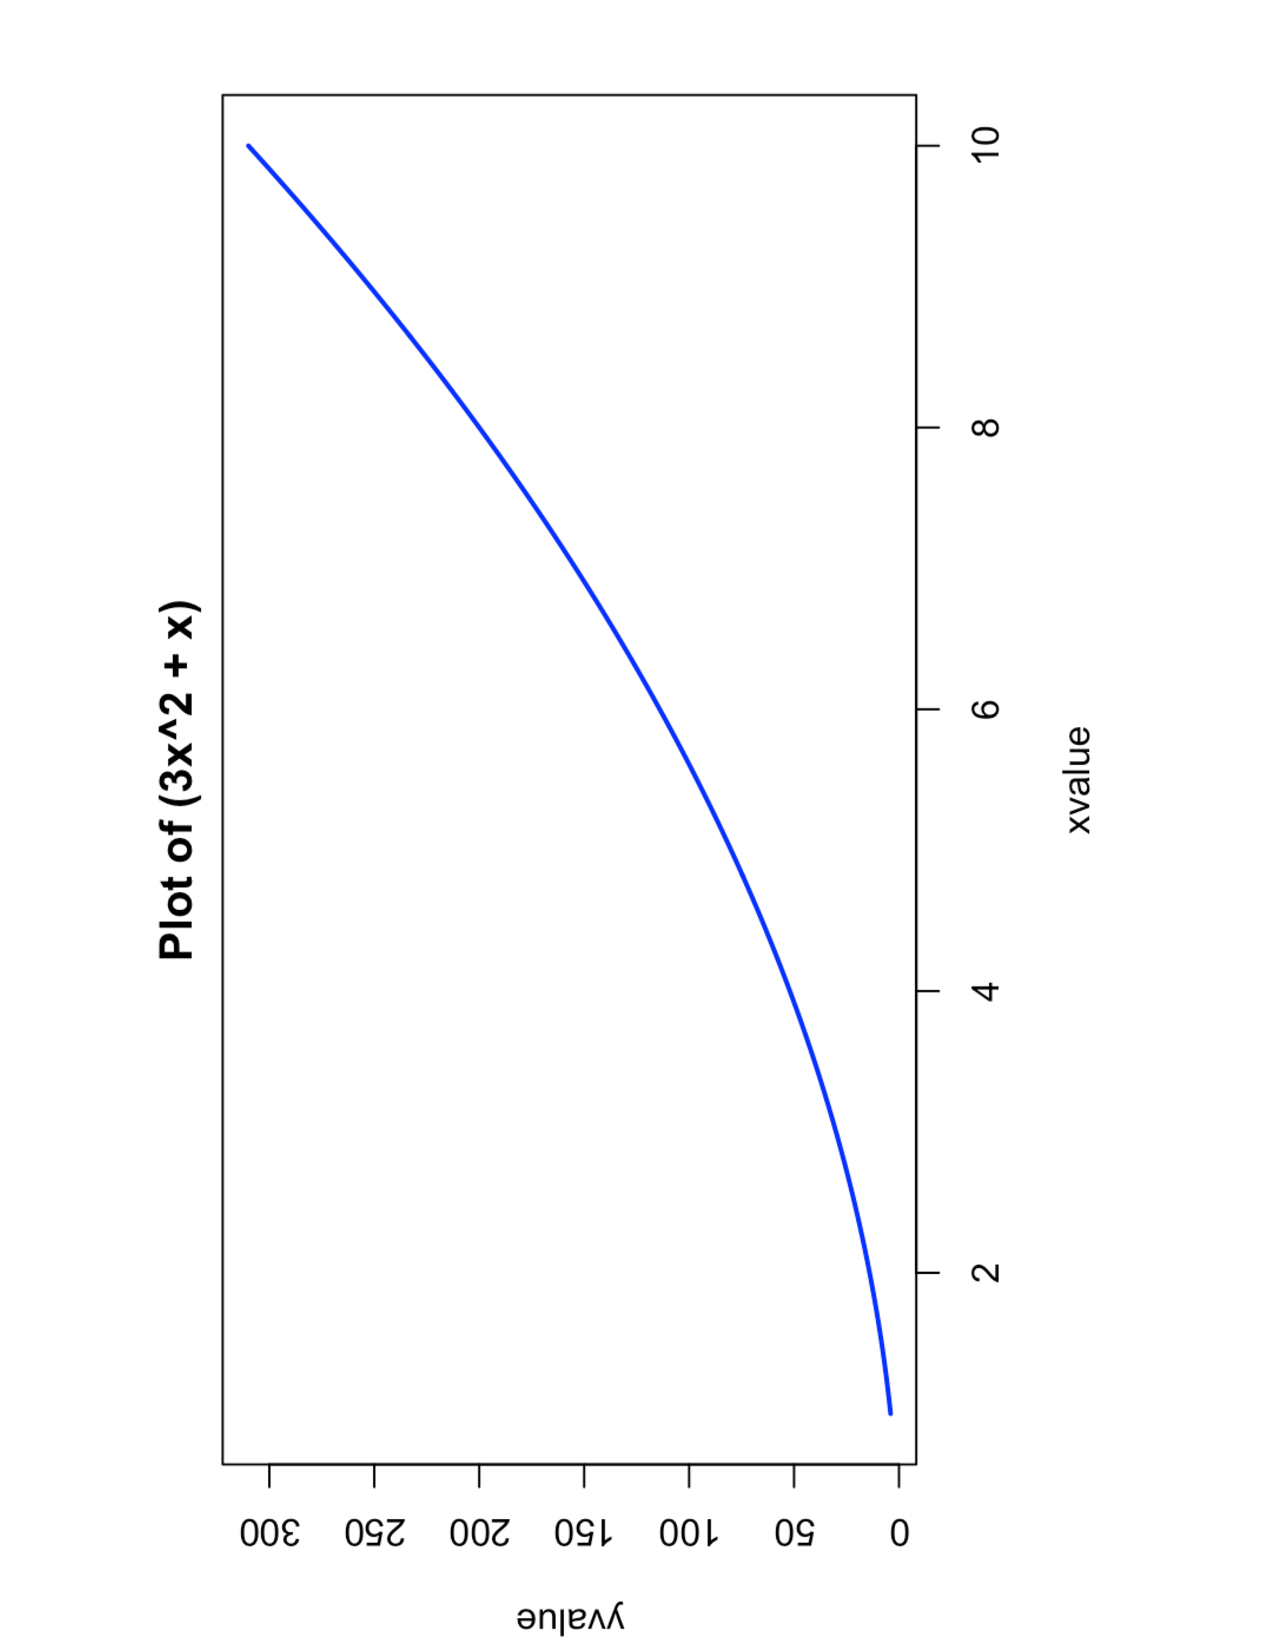
\includegraphics[width=\textwidth]{figure.pdf}
  \caption{This is my first figure.}
  \label{fig:graph}
\end{figure}

\section{Discussion}
\label{sec:disc}

What are the main contributions again?

What are the limitations of this study?

What are worth pursuing further in the future?

\lipsum[1-2]

\bibliography{refs}
\bibliographystyle{chicago}

\end{document}